\section{Evaluation}
\label{sec:evaluation}
Our system needs be suitable for economical use. This can be expressed as two requirements: On the one hand, the found joint NER and NEL process should find as many correct references as possible to organizations. While Ehmüller~\cite{ehmueller} evaluates this in terms of the standard measures precision, recall and $F_1$ score, I focus on how significant the features are without considering a certain classifier model. On the other hand, our system has to be capable of processing large amounts of data in reasonable time. As our project aims on solving this by means of cluster computing, I will evaluate how well the described preprocessing scales out.



\subsection{Significance of the features}
Given a link candidate $lc=(a, c)$ consisting of an alias $a$ and its context $c$ and an entity $en$, the classifier decides whether $lc$ references $en$ or not. Note that, while the link candidate's entity score $es_{en}(a)$ and the context score $cs_{en}(c)$ depend on $en$, $ls(a)$ only depends on the alias itself. Therefore these features must allow a distinction between valid and invalid links regarding the given entity. In the following, I evaluate the distribution of the features based on a sample of 100,000 composite features and how expressive they are for this distinction.

\begin{figure}
	\begin{tabular}{cc}
	\subfloat[Composite distribution of the entity score and the context score]{
		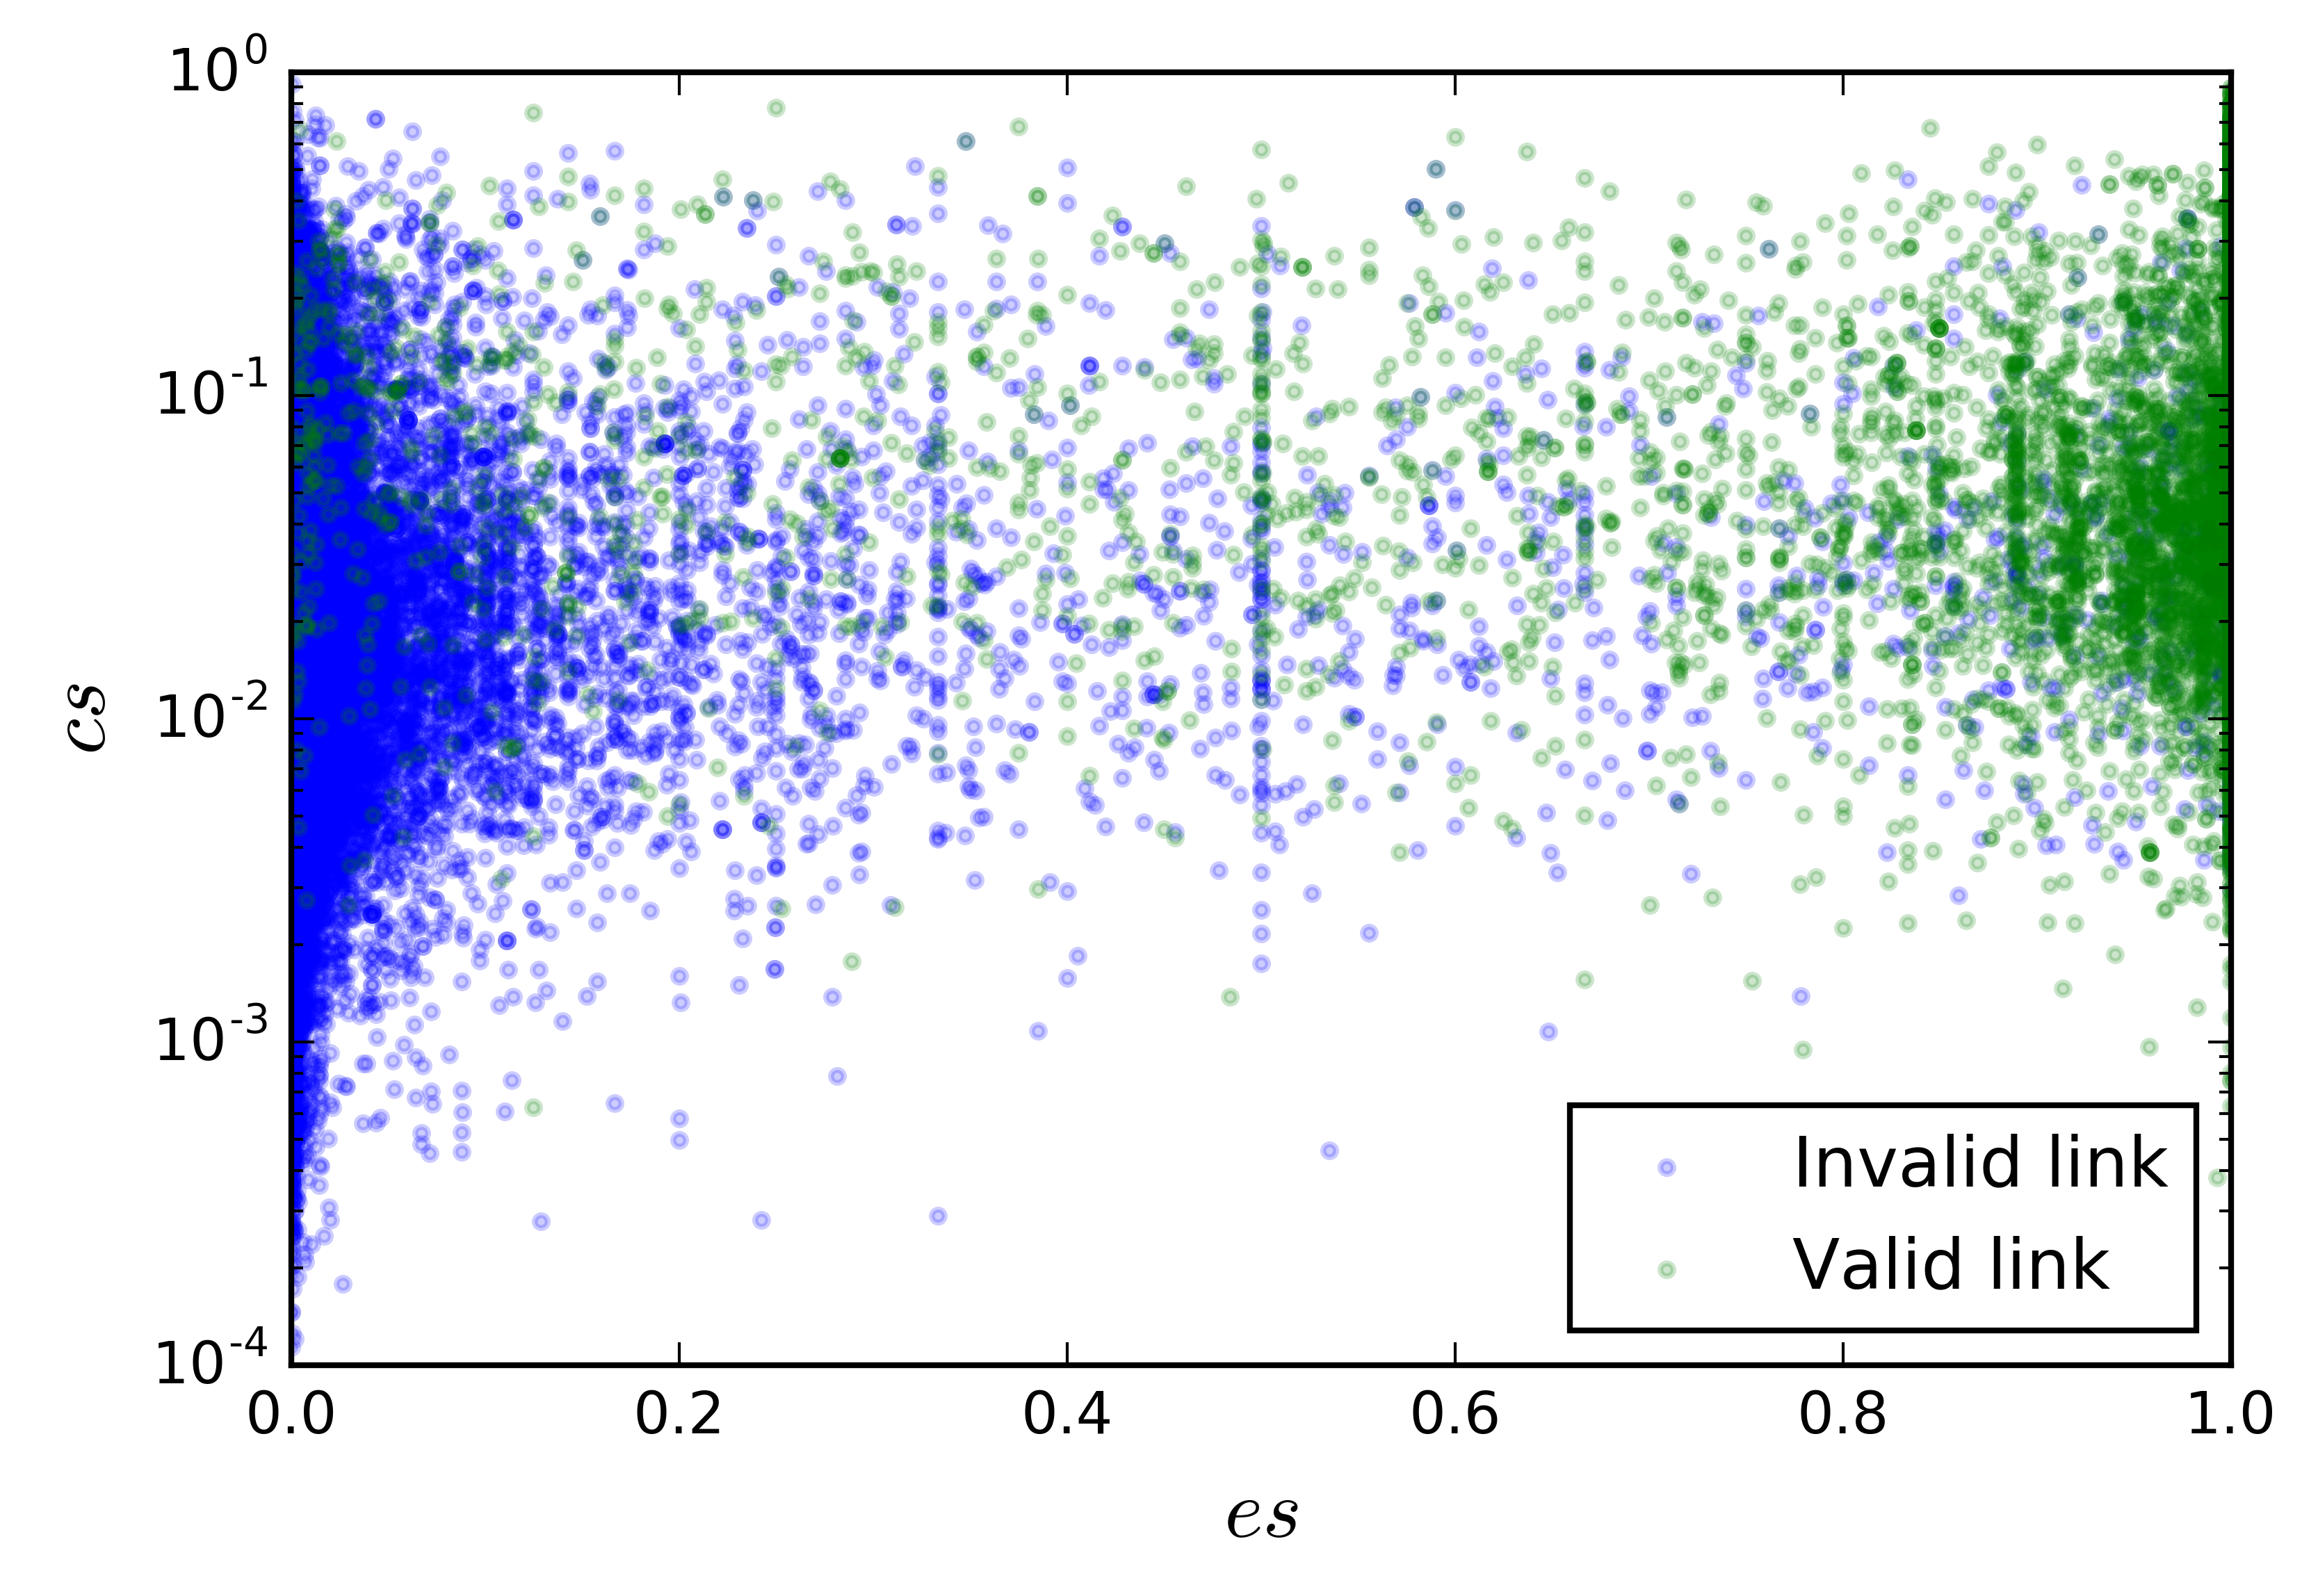
\includegraphics[width = 0.45\textwidth]{Graphics/feature_evaluation/composite_features.png}
		\label{fig:composite_features}
	} &
	\subfloat[Distribtion of the link scores]{
		\includegraphics[width = 0.45\textwidth]{Graphics/feature_evaluation/link_scores.pdf}
		\label{fig:link_scores}
	}\\
	\subfloat[Distribtion of the entity scores]{
		\includegraphics[width = 0.45\textwidth]{Graphics/feature_evaluation/entity_scores.pdf}
		\label{fig:entity_scores}
	} &
	\subfloat[Distribtion of the context scores]{
		\includegraphics[width = 0.45\textwidth]{Graphics/feature_evaluation/context_scores.pdf}
		\label{fig:context_scores}
	}
	\end{tabular}
	\caption{The valid and invalid links / no links have significantly different distributions of the three used features.}
	\label{fig:distributions}
\end{figure}

Figure~\ref{fig:composite_features} gives an overview about the composite distribution of the entity score and context score. Note that the context score is scaled logarithmically. The diagram reveals three properties:

\begin{enumerate}
\item There are two clearly identifiable \textbf{clusters}: One for valid links and a high entity score and one for invalid links and a low entity score. 

\item The entity score is more expressive than the context score, as the clusters can only be separated by means of the entity score.

\item There is a \textbf{correlation} between the entity score and the context score: There are far more valid links in the upper right half than in the lower left half of the diagram. This means, that the entity score and context score are "`confirming"' each other.
\end{enumerate}

Now we consider the features separately to get a more concise understanding of their quality:

\paragraph{Link score}
Figure~\ref{fig:link_scores} shows the distribution of the link scores for the valid and invalid links. Here and in the following, the overlap between the bars is shaded in dark blue. As not more than one entity is valid for each link candidate, our sample contains only 8\% valid links. Thus, for the better visibility, $f$ shows the relative frequency that is 1 both for the valid and invalid links when added up. We can see that a valid link has a link score that is close to 1 in more than 60\% of cases, while invalid links have a link score that is widely distributed. In fact, almost all of the links represented by the last bar have a link score, which is exactly 1. For the classifier, this means that

\paragraph{Entity score}
Figure~\ref{fig:entity_scores} shows the distribution of the entity scores. he extreme left and extreme right bar represent the clusters observed in Figure~\ref{fig:composite_features}. Thus, the entity score is very expressive for our task. A classifier that decides based on a linear separation between these clusters should yield reasonable results. But since the of valid links is relatively small, this feature is not sufficient.

\paragraph{Context score}
Finally, figure~\ref{fig:context_scores} shows the distribution of the context scores. Note that the frequency is scaled logarithmically. Although there is a large overlap between the valid and the invalid links, the distribution of the valid links is significantly shifted to higher context scores. For a context score of about 0.1, the context score has the least significance. The smaller or higher it becomes from there, the better the classifier can make its decisions.

\paragraph{Second order features}
Also the second order features have a high expressiveness, as shown in Figure~\ref{fig:second_order_features} in the appendix. Similar to the three features described above, they show significantly different distributions for valid and invalid links. Combined with them, the classifier improves the results of our NEL even further.


\subsection{Scale out}
Our context extraction and tf-idf computation is 1.30 times faster than the implementation of the Spark MLlib.\\
